% FortySecondsCV LaTeX template
% Copyright © 2019 René Wirnata <rene.wirnata@pandascience.net>
% Licensed under the 3-Clause BSD License. See LICENSE file for details.
%
% Attributions
% ------------
% * fortysecondscv is based on the twentysecondcv class by Carmine Spagnuolo 
%   (cspagnuolo@unisa.it), released under the MIT license and available under
%   https://github.com/spagnuolocarmine/TwentySecondsCurriculumVitae-LaTex
% * further attributions are indicated immediately before corresponding code


%-------------------------------------------------------------------------------
%                             ADDITIONAL PACKAGES
%-------------------------------------------------------------------------------
\documentclass[
  a4paper, 
%   showframes,
%   maincolor=cvgreen,
%   sectioncolor=red,
%   subsectioncolor=orange
%   sidebarwidth=0.4\paperwidth,
%   topbottommargin=0.03\paperheight,
%   leftrightmargin=20pt
]{fortysecondscv}

\usepackage{pdfpages}

% improve word spacing and hyphenation
\usepackage{microtype}
\usepackage{ragged2e}

% take care of proper font encoding
\ifxetex
	\usepackage{fontspec}
	\defaultfontfeatures{Ligatures=TeX}
% \newfontfamily\headingfont[Path = fonts/]{segoeuib.ttf} % local font
\else
	\usepackage[utf8]{inputenc}
	\usepackage[T1]{fontenc}
% \usepackage[sfdefault]{noto} % use noto google font
\fi

% enable mathematical syntax for some symbols like \varnothing
\usepackage{amssymb}

% bubble diagram configuration
\usepackage{smartdiagram}
\smartdiagramset{
  % defaut font size is \large, so adjust to harmonize with sidebar layout
  bubble center node font = \footnotesize,
  bubble node font = \footnotesize,
  % default: 4cm/2.5cm; make minimum diameter relative to sidebar size
  bubble center node size = 0.4\sidebartextwidth,
  bubble node size = 0.25\sidebartextwidth,
  distance center/other bubbles = 1.5em,
  % set center bubble color
  bubble center node color = maincolor!70,
  % define the list of colors usable in the diagram
  set color list = {maincolor!10, maincolor!40,
  maincolor!20, maincolor!60, maincolor!35},
  % sets the opacity at which the bubbles are shown
  bubble fill opacity = 0.8,
}

\usepackage{datetime}
\usepackage{lipsum}

%-------------------------------------------------------------------------------
%                            PERSONAL INFORMATION
%-------------------------------------------------------------------------------
% profile picture
\cvprofilepic{ValeLuca-29.jpg}
% your name
\cvname{Luca Di Stasio}
% job title/career
\cvjobtitle{Early Stage Researcher}
\cvcert{D-CPR Certified (FR, SE)}
\cvdlic{Driver License Cat. B (IT)}
\cvnation{Italian \& EU citizen}
% short address/location, use \newline if more than 1 line is required
\cvaddress{Stormv\"agen 299\newline SE-97634 Lule\aa, Sweden}
% phone number
\cvphone{+46 76 453 21 60}
% personal website
\cvsite{\href{https://www.lucadistasioengineering.com}{www.lucadistasioengineering.com}}
% email address
\cvmail{luca.distasio@gmail.com}
%\cvmailprof{luca.distasio@ingpec.eu}
%\linkedin{https://www.linkedin.com/in/lucadistasio/}{My Linkedin}
%\researchgate{https://www.researchgate.net/profile/Luca\_Di\_Stasio2}{My Researchgate}
%\github{https://github.com/LucaDiStasio}{My Github}

% add additional information
% \newcommand{\additional}{some more?}


%-------------------------------------------------------------------------------
%                              SIDEBAR 1st PAGE
%-------------------------------------------------------------------------------
% overwrite default icons and order of personal information
% \renewcommand{\personaltable}{%
% 	\begin{personal}[0.8em]
% 		\circleicon{\faKey}      & \cvkey  \\
% 		\circleicon{\faAt}       & \cvmail \\
% 		\circleicon{\faGlobe}    & \cvsite \\
% 		\circleicon{\faPhone}    & \cvphone \\
% 		\circleicon{\faEnvelope} & \cvaddress \\
% 		\circleicon{\faInfo}     & \cvbirthday \\
% 		% add another line
% 		\circleicon{\faQuestion} & \additional
% 	\end{personal}
% }

% add more profile sections to sidebar on first page
\addtofrontsidebar{
		
         	\profilesection{Contents}
		\skill{\textbf{p. 1}}{\hrulefill}
		\skill{\faBook}{Background}
		\skill{\faBook}{Higher Education Courses and Study Programmes}
		\skill{\textbf{p. 2}}{\hrulefill}
		\skill{\faBook}{Experience of Teaching and Supervision within Higher Education}
            \skill{\textbf{p. 3}}{\hrulefill}
		\skill{\faBook}{Pedagogic Activities: Description, Reflection and Development}
            \skill{\textbf{p. 6}}{\hrulefill}
		\skill{\faBook}{Development of Teaching Materials and Student Learning Resources}
		\skill{\faBook}{Experience of Leading, Administering and Developing Courses and Study Programs}
		\skill{\faBook}{Development, Depth of Study, Research and Dissemination of Knowledge}
		\skill{\faBook}{Pedagogic Activities outside the University}
	    \skill{\textbf{p. 7}}{\hrulefill}
		\skill{\faBook}{Annex A - Certificate of Completion: Qualifying Course for University Teachers}
	    \skill{\textbf{p. 9}}{\hrulefill}
		\skill{\faBook}{Annex B - Accepted Contribution to the Development Conference for Swedish Engineering Education 2019}
	    \skill{\textbf{p. 12}}{\hrulefill}
		\skill{\faBook}{Annex C - Final Course Assignment: Qualifying Course for University Teachers}
}


%-------------------------------------------------------------------------------
%                              SIDEBAR 2nd PAGE
%-------------------------------------------------------------------------------
\addtobacksidebar{
\profilesection{Contents}
		\skill{\textbf{p. 1}}{\hrulefill}
		\skill{\faBook}{Background}
		\skill{\faBook}{Higher Education Courses and Study Programmes}
		\skill{\textbf{p. 2}}{\hrulefill}
		\skill{\faBook}{Experience of Teaching and Supervision within Higher Education}
            \skill{\textbf{p. 3}}{\hrulefill}
		\skill{\faBook}{Pedagogic Activities: Description, Reflection and Development}
            \skill{\textbf{p. 6}}{\hrulefill}
		\skill{\faBook}{Development of Teaching Materials and Student Learning Resources}
		\skill{\faBook}{Experience of Leading, Administering and Developing Courses and Study Programs}
		\skill{\faBook}{Development, Depth of Study, Research and Dissemination of Knowledge}
		\skill{\faBook}{Pedagogic Activities outside the University}
	    \skill{\textbf{p. 7}}{\hrulefill}
		\skill{\faBook}{Annex A - Certificate of Completion: Qualifying Course for University Teachers}
	    \skill{\textbf{p. 9}}{\hrulefill}
		\skill{\faBook}{Annex B - Accepted Contribution to the Development Conference for Swedish Engineering Education 2019}
	    \skill{\textbf{p. 12}}{\hrulefill}
		\skill{\faBook}{Annex C - Final Course Assignment: Qualifying Course for University Teachers}
}

%\newdateformat{monthdayyeardate}{\monthname[\THEMONTH]~\THEDAY, \THEYEAR}%

\pagenumbering{arabic}
%-------------------------------------------------------------------------------
%                         TABLE ENTRIES RIGHT COLUMN
%-------------------------------------------------------------------------------
\begin{document}

\makefrontsidebar

\hrulefill\hspace{5pt}\textbf{\thepage}

\subsection{Background}
I am currently employed as a full-time PhD candidate in Polymeric Composite Materials at the Division of Materials Science, Department of Engineering Sciences and Mathematics, Lule\aa\ tekniska universitet (LTU) in Lule\aa, Sweden. I teach in 4 graduate-level courses offered in the subject of Polymeric Composite Materials. The courses are offered as part of the LTU-offered Master programme in Composite Materials and the international joint Master programmes in Materials Science and Engineering EEIGM/EUSMAT (European School of Materials Science and Engineering) and AMASE (Advanced Materials Science and Engineering).\\ Previously, I taught at the \'Ecole Europ\'eenne d'Ing\'enieurs en G\'enie des Mat\'eriaux (EEIGM) in Nancy, France in undergraduate- and graduate-level courses in Solid Mechanics, Viscoelasticity, Linear Elastic Fracture Mechanics, Mechanics of Composite Materials.\\I also contribute to the research activities of the Polymeric Composite Materials subject at LTU, working on integrated computational and experimental mechanics of polymers and polymer composites with a focus on fatigue, fracture and damage (see my Research Statement for more details).\\In addition, I am involved in the supervision of graduate students in the context of Master theses and project courses. I am actively involved in the continuous improvement of teaching practices in the subject of Polymeric Composite Materials by proposing new experimental activities for students (composites repair laboratory, bi-axial strain gauge measurements) as well as improving the virtual learning space of the courses offered in the subject. Furthermore, I actively contribute to the pedagogical research in Higher Education; currently I am working on a contribution (article and oral presentation) to the upcoming \textit{Development Conference for Swedish Engineering Education 2019}.

\subsection{Higher Education Courses and Study Programmes}
\textbf{Subject Related Courses}\\
As detailed in my resum\'e, I have received a BSc in Aerospace Engineering (2010) from Politecnico di Milano (Milan, Italy), a MSc in Mechanical Engineering (2012) from Drexel University (Philadelphia, USA), a MSc in Space Engineering (2013) from Politecnico di Milano (Milan, Italy), a PhD in Materials Science and Engineering (exp. Dec. 2019) from Universit\'e de Lorraine (Nancy, France) and a PhD in Polymeric Composite Materials (exp. Dec. 2019) from Lule\aa\ tekniska universitet (Lule\aa, Sweden).\\The courses I attended in these programs qualify me to teach within the specializations of Polymeric Composite Materials, Computational Mechanics, Experimental Mechanics, Computational Materials Science. I have also published peer-reviewed journal articles and conference papers and given several oral presentations in international conferences and seminars on Polymeric Composite Materials and Computational Mechanics (see my full list of publications for a more detailed account).\\[2pt]
\textbf{Pedagogic Courses}\\
I have successfully completed the 7.5 ECTS course \emph{Qualifying course for university teachers} at Lule\aa\ tekniska universitet (Lule\aa, Sweden) in February 2019.\\During my stay at the \'Ecole Europ\'eenne d'Ing\'enieurs en G\'enie des Mat\'eriaux (EEIGM) in Nancy, France, I also completed the following courses (in-presence or online) on Higher Education: Teaching in Higher Education (4 ECTS), Teaching Sustainability and Sustainable Development (2 ECTS), Oral Communication and Body Language in the Workplace (3.5 ECTS).\\Furthermore, in 2017 I completed the \textit{Software Carpentry Instructor Training Program} proposed by \textit{The Carpentries} to become a Certified Workshop Instructor. \textit{The Carpentries} is non-profit association whose aim is to teach software development and data science skills to researcher and to promote Open Science values and best practices.

\newpage
\makebacksidebar
\hrulefill\hspace{5pt}\textbf{\thepage}

\subsection{Experience of Teaching and Supervision within Higher Education}
\textbf{Teaching}\\[6pt]
\textit{Solid Mechanics, \'Ecole Europ\'eenne d'Ing\'enieurs en G\'enie des Mat\'eriaux (Nancy, France), 2017, Spring Term, Bachelor's Level ($2^{nd}$ year)}\\
I was in charge of the laboratory sessions devoted to tensile testing of aluminum, strain gauge measurements and thermomechanical measurements. I was also responsible for the examination (oral exam) and grading on this part of the course.\\[6pt]
\textit{Mechanics of Materials I, \'Ecole Europ\'eenne d'Ing\'enieurs en G\'enie des Mat\'eriaux (Nancy, France), 2017, Autumn Term, Bachelor's Level ($3^{rd}$ year)}\\
I taught tutorials to groups of 15-20 students on problems of viscoelasticity and linear elastic fracture mechanics in the form of interactive problem solving sessions. I also conducted workshops on the use of Finite Elements in materials modeling using the software Abaqus to groups of 15-20 students.\\[6pt]
\textit{Composite Materials, \'Ecole Europ\'eenne d'Ing\'enieurs en G\'enie des Mat\'eriaux (Nancy, France), 2017, Autumn Term, Master's Level ($1^{st}$ year)}\\
I conducted workshops on the use of Finite Elements in composite materials modeling using the software Abaqus to groups of 15-20 students.\\[6pt]
\textit{T7020T - Composites: Design and Numerical Methods, 7.5 ECTS, Lule\aa\ tekniska universitet (Lule\aa, Sweden), 2018, Autumn Term, Master's Level}\\
I was responsible for the laboratory sessions devoted to Mode I delamination testing (Double Cantilever Beam) of composites and calculation of Uni-Directional (UD) elastic properties from experimental data.\\[6pt]
\textit{T7005T - Aerospace Materials, 7.5 ECTS, Lule\aa\ tekniska universitet (Lule\aa, Sweden), 2018 - 2019, Spring Term, Master's Level ($1^{st}$ year)}\\
The course was divided into 3 main thematic sections: fatigue, fracture and damage in fiber-reinforced composites; joining techniques for composites; advanced metallic alloys. The first part, on fatigue, fracture and damage of composites, involved laboratory sessions of which I was in charge. In the 2019 edition of the course, I also defined the research topic of the laboratory session and designed the corresponding learning activities. I also improved the virtual learning space of the course by restructuring its content and appearance. Furthermore, I helped the design of the seminar activity in the section on advanced metallic alloys.\\[6pt]
\textit{T7012T - Composite Materials, 7.5 ECTS, Lule\aa\ tekniska universitet (Lule\aa, Sweden), 2018 - 2019, Autumn and Winter Term, Master's Level ($1^{st}$ year)}\\
I was responsible for the laboratory sessions devoted to manual manufacturing of composites, mechanical testing and calculation of Uni-Directional (UD) elastic properties from experimental data.\\[6pt]
\textit{T7011T - Mechanics of Fiber Composites, 7.5 ECTS, Lule\aa\ tekniska universitet (Lule\aa, Sweden), 2019, Winter Term, Master's Level ($1^{st}$ year)}\\
I was in charge of the laboratory sessions devoted to mechanical testing of composites and calculation of Uni-Directional (UD) elastic properties from experimental data.\\[6pt]
%%%%%%%%%%%
\textbf{Supervision}\\[6pt]
\underline{\emph{Bachelor and Master's theses and project courses}}\\[6pt]
\textit{E7009T - Degree Project, Materials Technology, 30 ECTS, Lule\aa\ tekniska universitet (Lule\aa, Sweden) and Universit\'a di Padova (Padova, Italy), 2019, Spring Term, Master's Level ($2^{nd}$ year)}\\
I co-supervised the Master's thesis work of an exchange student from Universit\'a di Padova (Padova, Italy). I met the student for 2-3 hours every week over 4 months and supported his activity by introducing him to experimental techniques, methods of design of experiments, programming languages and data analysis strategies. The student and I met with the main supervisor at Lule\aa\ tekniska universitet once every month.\\[6pt]
\textit{T7009T - Project Course, Materials Science and Engineering, 30 ECTS, Lule\aa\ tekniska universitet (Lule\aa, Sweden), 2019, Autumn Term, Master's Level ($2^{nd}$ year)}\\
I co-supervised the Project Course work of a Master level student. I formulated the research question of the project and designed the main learning activities.\\

\newpage
\makebacksidebar
\hrulefill\hspace{5pt}\textbf{\thepage}

\subsection{Pedagogic Activities: Description, Reflection and Development}
\textbf{Teaching Excellence: a Model of Target Attributes}\\[6pt]
At the beginning of my journey as a teacher in Higher Education, my original Model of Teaching Excellence was built upon my personal experience as a student and as a teacher. Being an Excellent Teacher, as I envisioned it, was thus to be the teacher I would have loved to meet when I was a student. That was the teacher I tried to be working with my first students. It was the product of my personal reflection over my experience, but no pedagogical foundation was present. A set of 8 attributes described this model of Excellent Teacher, ordered from the most to the least needed: empathic, understanding, respectful, listener, communicator, open-minded, life-long learner, expert. It was the image of a University teacher who capable of seeing each student as a responsible adult, available to help, open to different perspective and her/himself a curious learner. Expertise, meant as the expertise in one’s own field of teaching, was a less salient trait, as subject-knowledge is an ephemeral skill (today's pace of progress requires life-long learning in the scientific and technical fields) and could be developed along the way.\\
This vision of Excellent Teacher resonated with Kierkegaard’s idea of learning facilitator~\cite{kierkegaard1859,kierkegaard1998}: “All genuine helping begins with humility before the person I want to help and therefore I must understand that helping is not to dominate, but to serve”.  His humanistic approach to teaching was an eye-opener and represented the first critical comparison between my personal reflection on experience and the pedagogical literature. From this first encounter with Higher Education pedagogy I gained confidence and, quite frankly, a sense of relief: my reflections were in agreement with other authors, they were not only my personal views! Such realization was for me especially important, as I had been growing professionally in technical environments where teaching is usually regarded as a minor duty.\\
Since then, my Model of Excellent Teaching and its Attributes have been evolving through a continuous comparison between experience in the classroom, personal reflection, study of pedagogical principles and experimentation of learning techniques. I currently envision the Excellent Teacher as: a counselor, an active listener, an open-minded person, a communicator, a life-long learner, a pedagogical expert and a team-player.\\
I believe that Maslow’s hierarchy of needs~\cite{maslow1954} represents a clear and workable reference model of an individual’s motivations to act, albeit not a complete or self-contained explanation of it. At the lower levels of Maslow's pyramid sit basic needs such as physiological ones (hunger, thirst, rest, ...) and physical safety; they are followed by psychological needs, expressed in the need of belonging, of having meaning relationship, of having self-esteem; learning belongs to the top, i.e. self-actualization, creativity, the need to fulfill one own's potential. Although the hierarchy should not be taken as a strict, one-way procedure to achieve self-fulfillement, it certainly grasps some important and, alas, often overlook workings of the human being: there exists a relation of urgency between needs and desires, and the lack of fulfillement of one level of the hierarchy affects the higher levels. Given that learning sits at the top, we can argument that learning is affected by feelings, physical and psychological. If a student feels discriminated, harassed or in danger, s/he will not perform well. The first duty of the teacher is to observe students and listen to them: hear their grievances and evaluate them fairly, investigate with tact situations of personal hardship and guide students to the right source of help (financial, psychological, physical, ...). It is in this sense that I view the Excellent Teacher as a counselor and an active listener: someone capable of listening and understanding students, guiding them to the right help, and ensuring that the learning environment is safe, fair, free from discrimination of any kind, open to all contributions.\\
In a more comprehensive way, the learning environment should should be inclusive. My understanding of the problem of inclusion starts by recalling the GAP model of disability~\cite{ahlmark}: a disability exists when there is a gap between an individual’s capabilities and demands from the environment. The teacher should be attentive to any case in which such gap between individual’s capabilities and learning activities’ requirements prevents the student from achieving the intended learning outcomes. Indeed in Sweden, where I am currently employed, the teacher is required to act in accordance to the Swedish Discrimination Act~\cite{discri2008} in the case the student reports a medically certified disability. However, in the perspective of the affective taxonomic domain~\cite{krathwohl1973}, I believe this is a low-level behavior: responding or committing to ideas, values, principles and actions as mandated by the law and by the role.\\

\newpage
\makebacksidebar
\hrulefill\hspace{5pt}\textbf{\thepage}

The Excellent Teacher should not be satisfied at this level: the aim should be the highest taxonomic level, i.e. internalization. The Excellent Teacher should be proactive, talk with students, listen to them, understand their problems and direct them to the most suited help available. The Excellent Teacher should at the same time respect students’ privacy and not be intrusive. The Excellent Teacher is, first and foremost, a counselor.\\
Feedback is in this sense the primary tool of the Excellent Teacher~\cite{elmgren2015}. Feedback represents the chance for the teacher to verify the alignment~\cite{elmgren2015} of the learning activity designed with the intended learning outcomes. For the student, feedback shows whether the effort spent has produced the expected learning, and how it should or could be improved. For the feedback to be effective, the teacher should listen and should understand what the student is communicating: understanding cannot be shallow (the mere literal meaning), but deep (the intended content). This is what is called “active listening” in the counseling community~\cite{knights1985,robertson2005} . The Excellent Teacher is not only a listene, but an active listener. On the other hand, to receive feedback and use it for improvement, the Excellent Teacher must be open to critiques on one's own work: the Excellent Teacher is open-minded.\\
Communication is thus at heart of the teaching activity: creation of a safe and welcoming environment, inclusion, feedback require good communication skills. The Excellent Teacher needs to be a good communicator.\\
Motivation is key to students’ engagement and focus~\cite{rust2013,ariely2008,yeager2014} and intrinsically motivated students tend to prefer deep approaches to learning~\cite{rust2013,yeager2014}. The best and probably simplest way for the teacher to relate to students’ intrinsic motivation is to show strong interest and passion for the subject taught, to present its links with the students’ future profession and today's world in general. This is achieved if the teacher is a life-long learner. It means that the teacher has a strong desire to learn and improve and that the teacher regards the teaching assignment first and foremost as a learning moment. Therefore, the Excellent Teacher is a life-long learner.\\
Effective design of learning activities is achieved by following the principles of constructive alignment\cite{schuel1986,biggs2003,wadsworth2004} and using tools such as the taxonomies\cite{krathwohl1973,anderson2001,dave1975}, Kolb’s cycle~\cite{kolb1984} and the ICAP framework~\cite{chi2014}. Pedagogical expertise is thus a fundamental skill of the teacher, who should be able to correctly formulate learning outcomes and design learning activities aligned with these outcomes. The Excellent Teacher should be a pedagogical expert. As design of learning activities very often occur in teams, being an Excellent Teacher implies being a team-player.\\[6pt]
\textbf{Future Work and Development}\\[6pt]
In the context of my pedagogical formation, I have developed a set of competencies of learner- (or learning-) centric design which I would like to put more deeply into practice. Although I have had certainly room to act in the context of my teaching assignments, wider and more drastic proposals will likely face the opposition of an environment in which the belief in traditional teacher-centric design is strong. I will need to motivate my ideas and proposals with results from the literature and from my experience, which will require a continuous work of recording students’ feedback and performance. I regard it as an interest challenge ahead of me, strictly related to the development of my teaching practice as documented by the portfolio.\\[6pt]

\newpage
\makebacksidebar
\hrulefill\hspace{5pt}\textbf{\thepage}

\textbf{References}

\renewcommand{\section}[2]{}
\begin{thebibliography}{9}

\bibitem{kierkegaard1859} 
Kierkegaard, S. (1859).
\textit{Synspunktet for min Forfatter-Virksomhed.: En ligefrem Meddelelse: Rapport till Historien.}
Kjöbenhavn: Reitzel.
 
\bibitem{kierkegaard1998} 
Kierkegaard, S. (1998).
\textit{The Point of View.}. [Translated by Hong, H. V. and Hong E. H.] 
Princeton, N.J. Princeton University Press.
 
\bibitem{maslow1954} 
Maslow, A. (1954).
\textit{Motivation and personality.}
New York, NY: Harper.

\bibitem{ahlmark} 
Ahlmark D. L.
\textit{Universal Design for Learning (UDL).}
Available at: https://ltu.instructure.com/courses/5889/pages/what-is-more-to-master-inclusion-1-5h?module\_item\_id=78900.

\bibitem{discri2008} 
\textit{Discrimination Act (2008:567).}
Available at: https://www.government.se/information-material/2015/09/discrimination-act-2008567/.

\bibitem{krathwohl1973} 
Krathwohl D. R., Bloom B. S., \& Masia B. B. (1973).
\textit{Taxonomy of educational objectives, the Classification of educational goals. Handbook II: Affective domain.}
New York: David McKay Co., Inc.

\bibitem{elmgren2015} 
Elmgren M., Henriksson A.-S. (2015).
\textit{Academic Teaching.}
Studentlitteratur, Lund.

\bibitem{knights1985} 
Knights S. (1985).
\textit{Reflection and learning: the importance of a listener.}
In: Reflection, turning experience into learning. Eds.: Boud D., Keogh R., Walker D. New York: Nichols Publishing Company.

\bibitem{robertson2005} 
Robertson K. (2005).
\textit{Active listening: More than just paying attention.}
Australian Family Physician, 34(12).

\bibitem{rust2013} 
Rust C. (2013).
\textit{What do we think we know about student learning, and what are the implications of improving that learning? Foreword.}
Improving Learning through Research and Scholarship. Oxford Brookes University. 

\bibitem{ariely2008} 
Ariely D.,  Kamenica E. and Prelec D. (2008).
\textit{The man’s search for meaning: the case of legos.}
Journal of Economic Behavior and Organisation, 67(3-4), 671-677.

\bibitem{yeager2014} 
Yeager D. S., Henderson M., Paunesku D., Walton G. M., D’Mello S., Spitzer B. J. and Duckworth A. L. (2014).
\textit{Boring but Important: A Self-Transcendent Purpose for Learning Fosters Academic Self-Regulation.}
Journal of Personality and Social Psychology, 107(4), 559-580.

\bibitem{schuel1986} 
Schuel T. J. (1986).
\textit{Cognitive Conceptions of Learning.}
Review of Educational Research, 56, 411-436.

\bibitem{biggs2003} 
Biggs. J. (2003).
\textit{Teaching for Quality Learning at University – What the Student Does (2nd Edition).}
SRHE / Open University Press, Buckingham.

\bibitem{wadsworth2004} 
Wadsworth B. J. (2004).
\textit{Piaget's theory of cognitive and affective development: Foundations of constructivism.}
Longman Publishing.

\bibitem{anderson2001} 
Anderson L. W., Krathwohl D. R. and Bloom B. S. (ed., 2001).
\textit{A taxonomy for learning, teaching, and assessing: a revision of Bloom’s taxonomy of educational objectives.}
New York: Longman.

\bibitem{dave1975} 
Dave R. H. (1975). Developing and Writing Behavioural Objectives. Ed.:  Armstrong R. J. Educational Innovators Press.

\bibitem{kolb1984} 
Kolb D. A. (1984).
\textit{Experiential learning: experience as the source of learning and development.}
New Jersey: Englewood Cliffs.

\bibitem{chi2014} 
Chi M. T. and Wylie R. (2014).
\textit{The ICAP framework: Linking cognitive engagement to active learning outcomes.}
Educational Psychologist, 49(4), 219-243.

\end{thebibliography}

\newpage
\makebacksidebar
\hrulefill\hspace{5pt}\textbf{\thepage}

\subsection{Development of Teaching Materials and Student Learning Resources}
\textit{T7005T - Aerospace Materials, 7.5 ECTS, Lule\aa\ tekniska universitet (Lule\aa, Sweden), 2018 - 2019, Spring Term, Master's Level ($1^{st}$ year)}\\
I participated in the preparation of the hand-out, in the form of a presentation, describing the tasks of the group-based project. I worked on improving the virtual learning space of the course by organizing its content and structuring its appearance.

\subsection{Experience of Leading, Administering and Developing Courses and Study Programs}
As part of the coursework for the 7.5 ECTS course \emph{Qualifying course for university teachers} at Lule\aa\ tekniska universitet (Lule\aa, Sweden), I re-designed the 7.5 ECTS course \textit{T7005T - Aerospace Materials} (see attachment for more details). To this end, I proposed a new format of flipped-classroom learning for the theoretical part of the course and a more articulated management of the group-based project. The core idea of this new design is to bring passive-active (with respect to the ICAP framework), lower taxonomy level activities outside of the classroom and focus the in-class work on constructive and interactive behaviors aimed to the construction of new knowledge. As this course is propedeutic to independent research projects in the last year of studies, the new version of the course would provide a fail-safe training ground similar to the daily activity of the researcher and the engineer, who develop projects with uncertain initial boundaries and need to interact with co-workers, team leaders, customers and stakeholders.

\subsection{Development, Depth of Study, Research and Dissemination of Knowledge}
I am currently preparing a contribution in the form of conference article and oral presentation, which has been accepted for the upcoming \textit{Development Conference for Swedish Engineering Education 2019} to be held at Lule\aa\ tekniska universitet (Lule\aa, Sweden) in November 2019. In this contribution I present, in the form of a work in progress, a reflection on the relation between the signature pedagogy of mechanics of materials and its threshold concepts, and I further propose a revised flipped-classroom format for lectures on mechanics of materials based on the signature pedagogy. In the long-term, the goal is to be experiment this revised flipped-classroom format in a course on mechanics of materials and verify its effectiveness through students' feedback and review from peers. The results would then be amenable for publication in a peer-reviewed international journal to get feedback from the wider community of practitioners in Higher Education.

\subsection{Pedagogic Activities outside the University}
I am an active member of the non-profit organization \emph{The Carpentries}, with which I collaborate on a volunteer basis. The main objective of the organization is to teach foundational skills in software development and data analysis to researchers and academics at all levels (from students to professors) and to promote Open Science values and best practices. To achieve this goal, it offers free online tutorials on different technical topics and organizes, upon request from local institutions, in-person workshops. To this end, the organization trains its volunteer members on active learning strategies. To distinguish members who have acquired such skills, \emph{The Carpentries} proposes a specific training path which, upon successful completion, provides the status of \emph{Certified Instructor} and the possibility to teach in workshops. I completed the instructor training in 2017 and I am, since then, a \emph{Certified Instructor}. In October 2018, I participated as main instructor in a Carpentry workshop offered by the High Performance Computing Center North (HPC2N) at Ume\aa\ University (Ume\aa, Sweden), where I taught the use of bash, bash scripting, Git and Github. In addition, I contributed to the development of the workshop lessons material, which is freely available on Github. I contributed also to a Task Force to develop recommendations on handling incidents outside the Code of Conduct of the \emph{The Carpentries}.

\newpage
\makebacksidebar
\hrulefill\hspace{5pt}\textbf{\thepage}

\subsection{Annex A}

\textbf{Certificate of Completion: Qualifying Course for University Teachers, 7.5 ECTS, Lule\aa\ tekniska universitet (Lule\aa, Sweden)}

\newpage
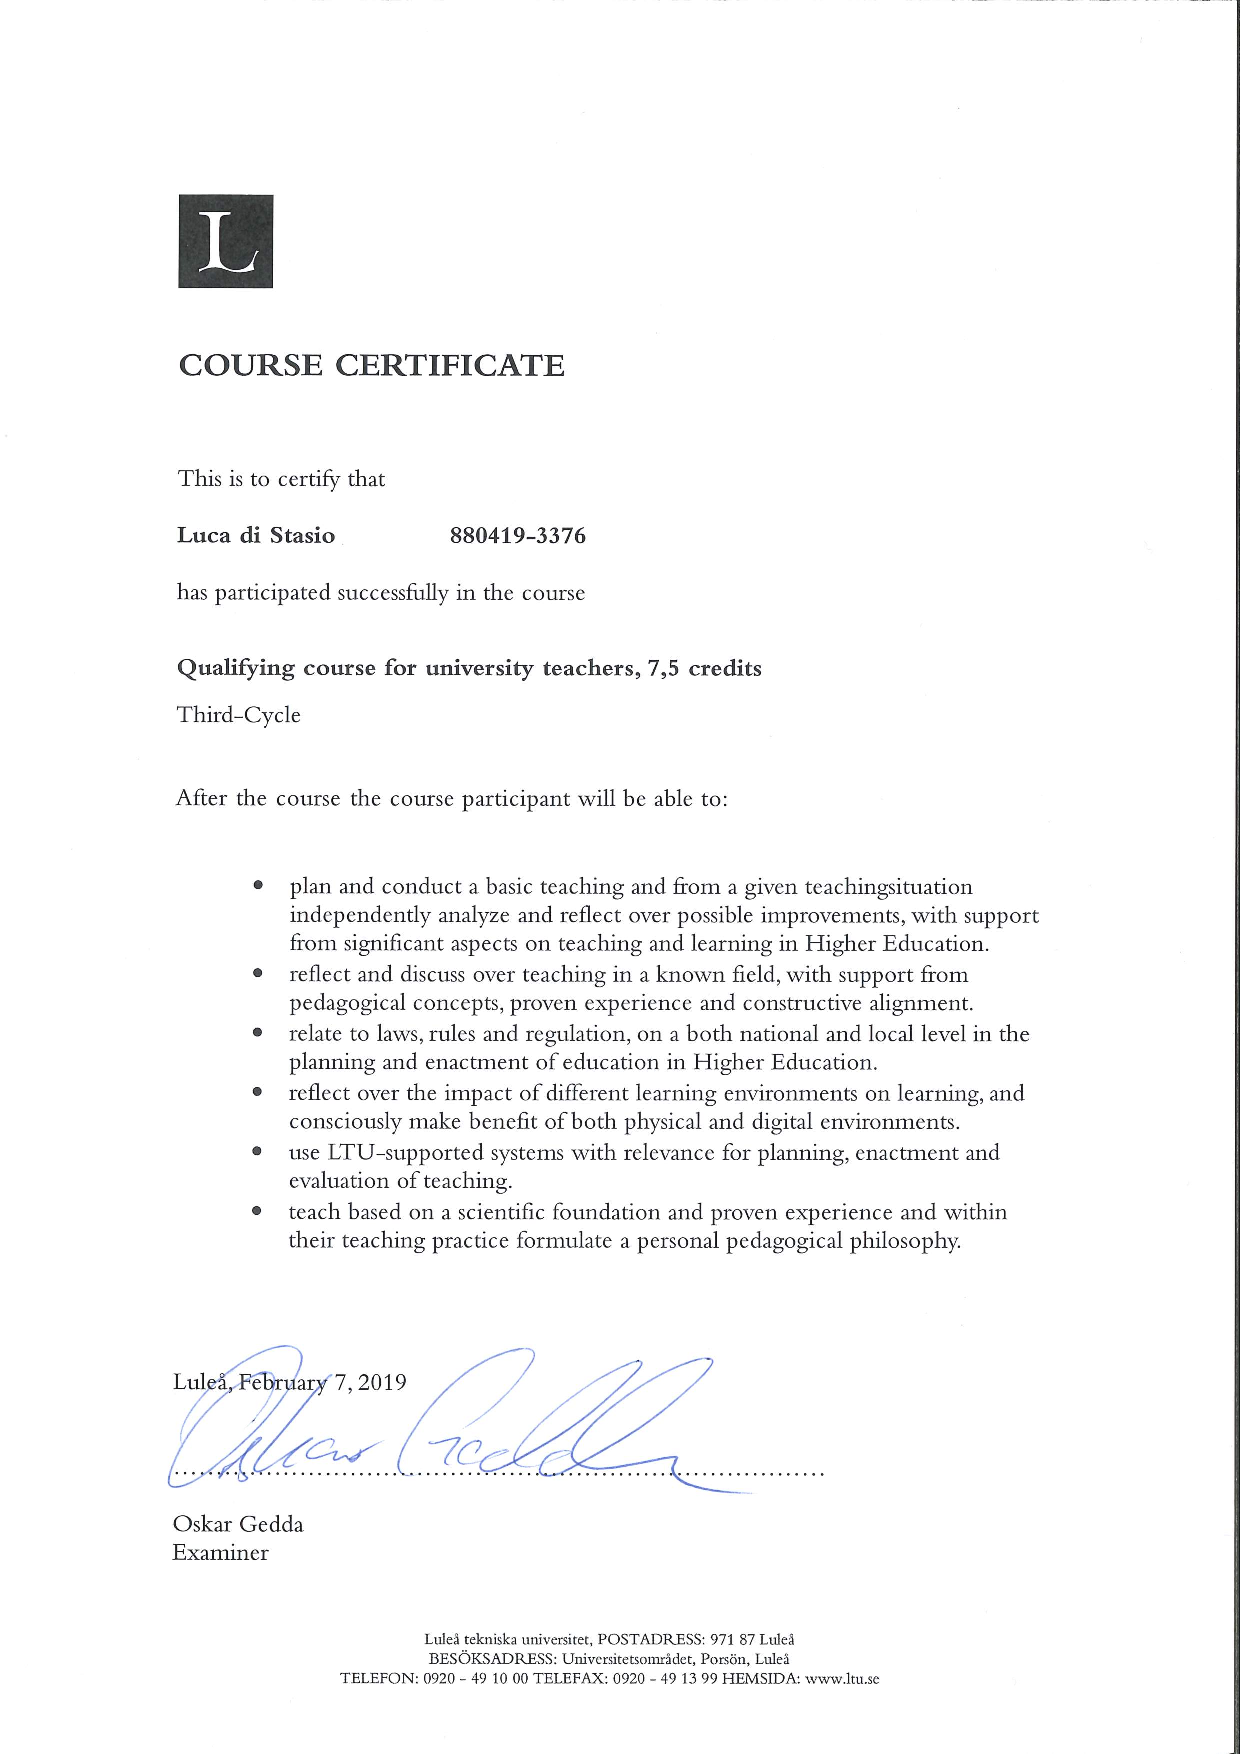
\includepdf[pages=-]{DiStasio-QCUT2018-Certificate.pdf}

\newpage
\makebacksidebar
\hrulefill\hspace{5pt}\textbf{\thepage}

\subsection{Annex B}

\textbf{Accepted Contribution to the Development Conference for Swedish Engineering Education 2019, November 2019, Lule\aa\ tekniska universitet (Lule\aa, Sweden)}

\newpage
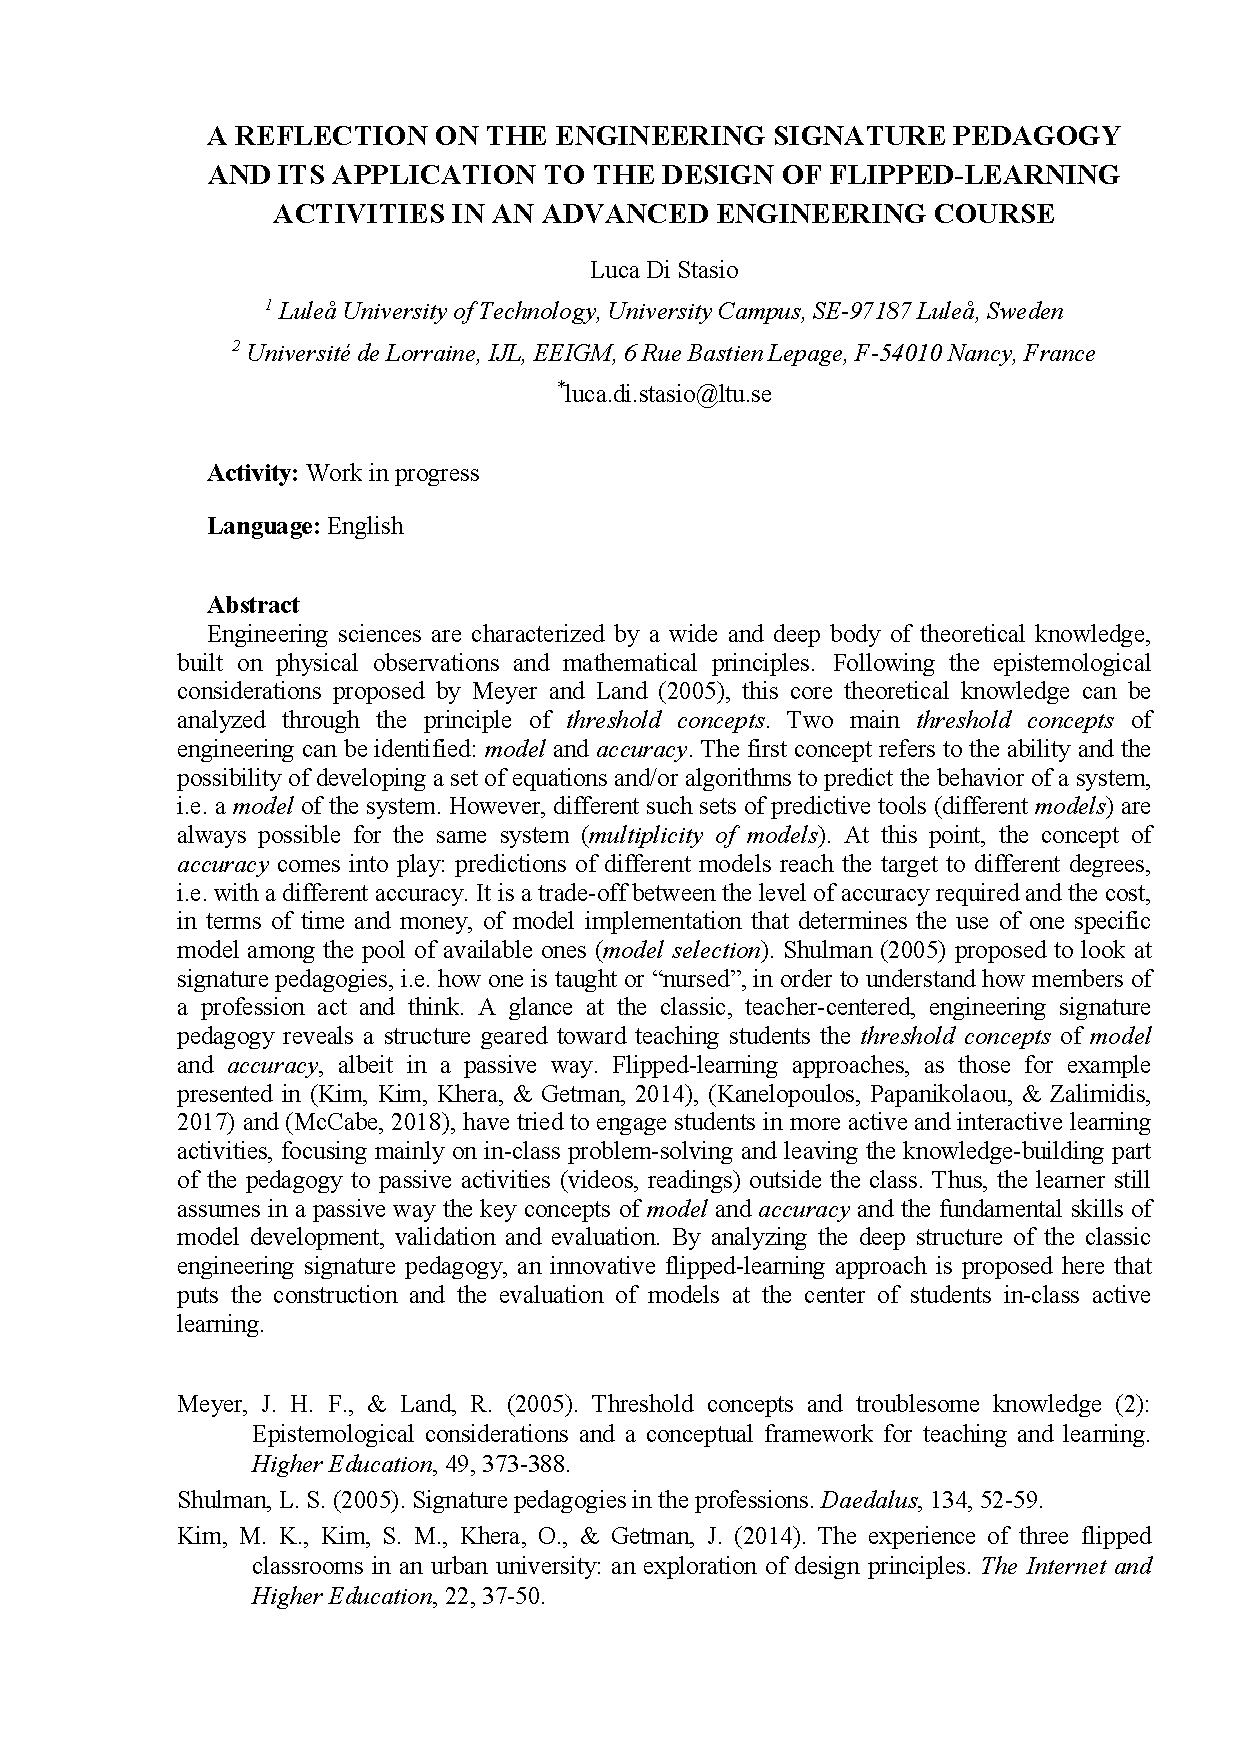
\includepdf[pages=-]{DevConfSweEngEdu2019.pdf}

\newpage
\makebacksidebar
\hrulefill\hspace{5pt}\textbf{\thepage}

\subsection{Annex C}

\textbf{Final Course Assignment: Qualifying Course for University Teachers, 7.5 ECTS, Lule\aa\ tekniska universitet (Lule\aa, Sweden)}

\newpage
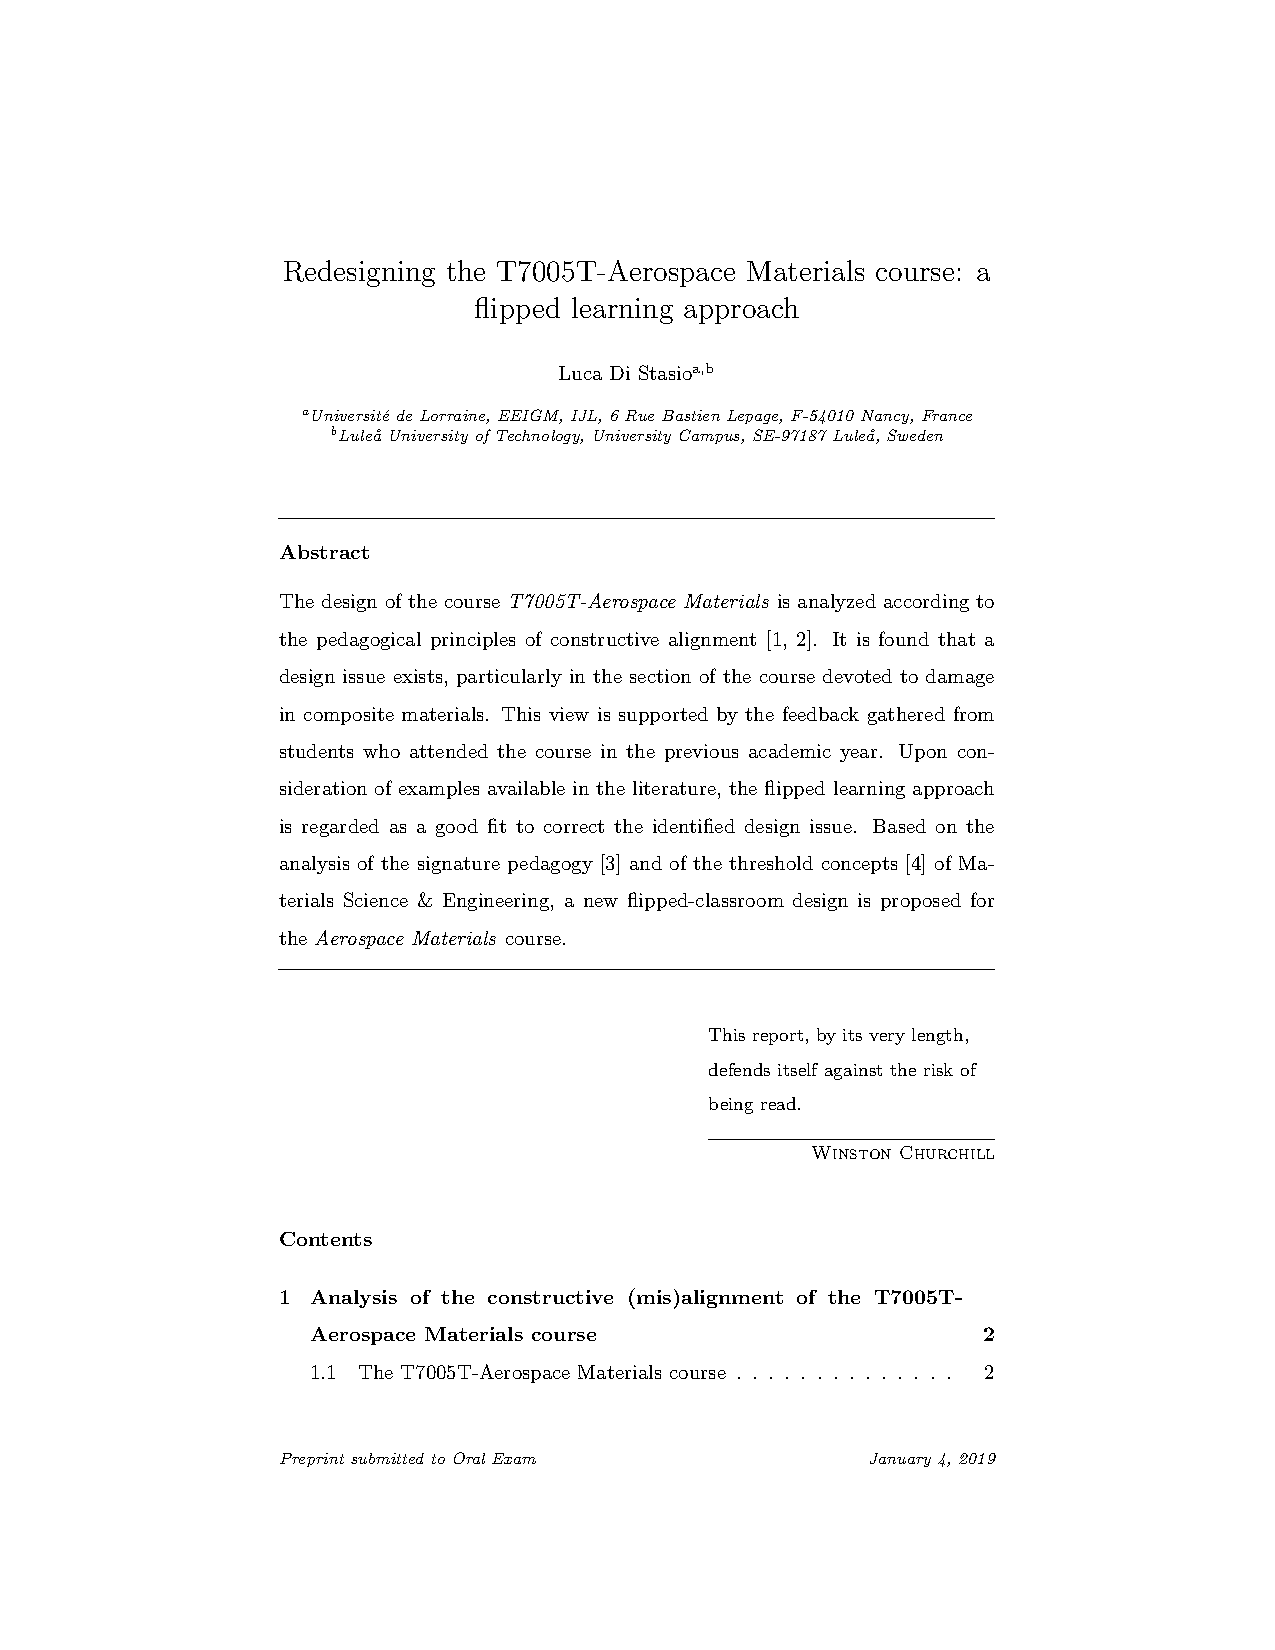
\includepdf[pages=-]{T7005T-flipped-design.pdf}

\end{document} 
